\section{Language Artificial Intelligence} % (fold)
\label{sec:language_ai}
%
\begin{frame}[t,fragile] \frametitle{Language AI}
    \framesubtitle{\ldots o NLP}
	{\small
	    \begin{minipage}[t]{\textwidth}
	    	\begin{itemize}[leftmargin=10pt,align=right]
				\onslide<1->\item[\alert{\faArrowCircleRight}] Sottocampo dell'AI dedicato allo sviluppo di tecnologie per il linguaggio umano
				\begin{itemize}[leftmargin=10pt,align=right]
					\item[\alert{\faArrowCircleRight}] Comprensione
					\item[\alert{\faArrowCircleRight}] Elaborazione
					\item[\alert{\faArrowCircleRight}] Generazione
				\end{itemize}
				\onslide<2->\item[\alert{\faArrowCircleRight}] Utilizzato intercambiabilmente con \alert{Natural Language Processing} (NLP)
				\onslide<3->\item[\alert{\faExclamationTriangle}] \alert{Trasversale} rispetto alla classificazione canonica
			\end{itemize}
	    \end{minipage}
	}
\end{frame}
%
\begin{frame}[t]
    \frametitle{Language AI}
    \framesubtitle{Esempi di \emph{task} NLP}
    {\scriptsize
        \begin{minipage}[t]{\textwidth}
            \begin{minipage}[t]{.33\textwidth}
                \begin{figure}[hb]
                    \centering
                    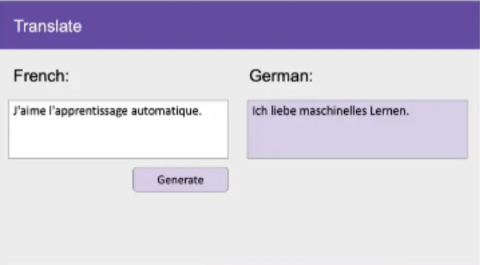
\includegraphics[width=\textwidth]{Translator.png}\\Traduzione \emph{context-sensitive}
                \end{figure}
            \end{minipage}
            \begin{minipage}[t]{.33\textwidth}
                \begin{figure}[hb]
                    \centering
                    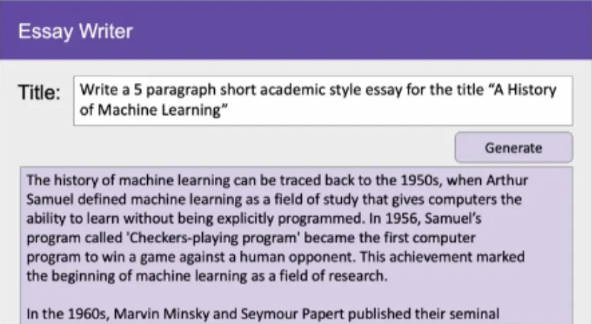
\includegraphics[width=\textwidth]{essay-writer.png}\\Generazione di testo
                \end{figure}
            \end{minipage}
            \begin{minipage}[t]{.33\textwidth}
                \begin{figure}[hb]
                    \centering
                    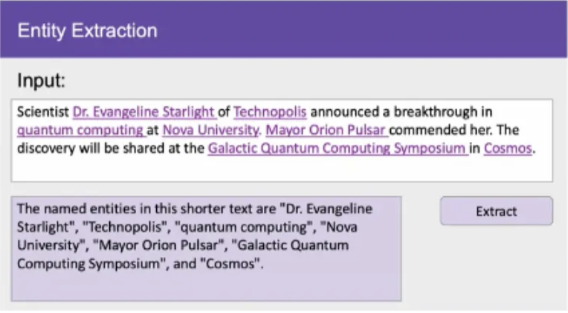
\includegraphics[width=\textwidth]{NER.png}\\Estrazione di entità denominate
                \end{figure}
            \end{minipage}
        \end{minipage}
    \\\vspace*{.5cm}
        \begin{minipage}[b]{\textwidth}
            \begin{minipage}[b]{.33\textwidth}
                \begin{figure}[hb]
                    \centering
                    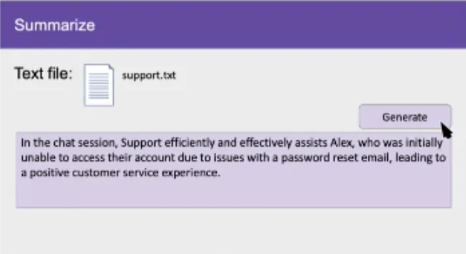
\includegraphics[width=\textwidth]{summarization.png}\\Riassunto di testi
                \end{figure}
            \end{minipage}
            \begin{minipage}[b]{.33\textwidth}
                \begin{figure}[hb]
                    \centering
                    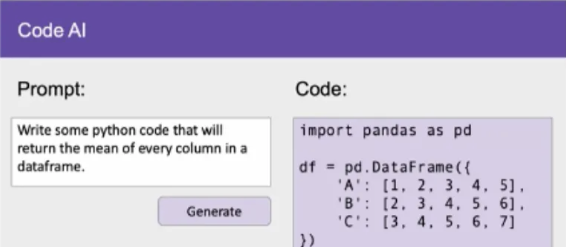
\includegraphics[width=\textwidth]{Code-generator.png}\\Generazione di codice
                \end{figure}
            \end{minipage}
            \begin{minipage}[b]{.33\textwidth}
                \begin{figure}[hb]
                    \centering
                    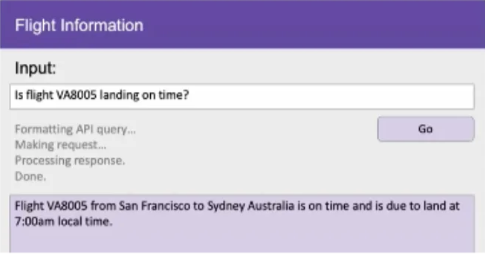
\includegraphics[width=\textwidth]{assistant.png}\\Assistente digitale
                \end{figure}
            \end{minipage}
        \end{minipage}
		\begin{center}
			\href{https://www.google.com}{\faExternalLinkSquare\ Gara GPT vs Claude su traduzione \textit{context-sensitive}}
		\end{center}
    }
\end{frame}
%
\begin{frame}[t]
    \frametitle{\emph{Language models}}
    \framesubtitle{$\ldots$ o modelli del linguaggio}
	\vspace*{-1cm}
	{\footnotesize 
        \begin{minipage}[t]{\textwidth}
            \vspace*{.5cm}
            \begin{itemize}[leftmargin=10pt,align=right]
				\onslide<1->\item[\alert{\faArrowCircleRight}] Modelli che simulano la comprensione e la generazione del linguaggio umano con approcci statistici e modelli della rete neurale
                \onslide<2->\item[\alert{\faArrowCircleRight}] Predicono la parola successiva in una sequenza in base al \alert{contesto}$\ldots$
                \onslide<3->\item[\alert{\faArrowCircleRight}] $\ldots$ calcolando probabilità su ogni singola parola di un \alert{dizionario}
                \onslide<4->\item[\alert{\faExclamationTriangle}] \alert{Qualunque} \emph{task} NLP può essere trasformata in un problema di generazione di testo!
            \end{itemize}
        \end{minipage}
		\hspace*{2cm}
		\only<4|handout:1>{
        \begin{minipage}[t]{.8\textwidth}
			\vspace*{.3cm}
			\renewcommand{\epigraphsize}{\scriptsize}
			\setlength{\afterepigraphskip}{5pt}
			\setlength{\beforeepigraphskip}{5pt}
			\setlength{\epigraphwidth}{\textwidth}
			\epigraph{\textit{\alert{\faUser\ (thinking)} --- Ho la frase <<Mi piace come recita Hugh Laurie!>>, e devo determinarne il \emph{sentiment} ---\\
			\alert{\faUser} ``Il \emph{sentiment} della frase <<Mi piace come recita Hugh Laurie!>> é: ''\\
			\alert{\faTerminal\ (thinking)} --- Eseguo l'inferenza\ldots ---\\
			\alert{\faTerminal\ (thinking)} --- Ho ottenuto le seguenti probabilità come prossimo \textit{token} da generare: <<positivo>> al 45\%, <<negativo>> al 2\%, <<cane>> al 0.5\%, <<gatto>> al 0.3\%,\ldots ---\\
			\alert{\faTerminal} ``Il \emph{sentiment} della frase <<Mi piace come recita Hugh Laurie!>> é: positivo''}}{\textbf{Processo di \textit{sentiment analysis}}}
        \end{minipage}
		}
		\only<5|handout:2>{
        \begin{minipage}[t]{.8\textwidth}
			\vspace*{.3cm}
			\renewcommand{\epigraphsize}{\scriptsize}
			\setlength{\afterepigraphskip}{5pt}
			\setlength{\beforeepigraphskip}{5pt}
			\setlength{\epigraphwidth}{\textwidth}
			\epigraph{\textit{\alert{\faUser\ (thinking)} --- Ho la domanda <<Chi ha scritto ``L'origine della specie''?>> e voglio ottenere la risposta ---\\
			\alert{\faUser} ``D: Chi ha scritto <<L'origine della specie>>? R: ''\\
			\alert{\faTerminal\ (thinking)} --- Eseguo l'inferenza\ldots ---\\
			\alert{\faTerminal\ (thinking)} --- Ho ottenuto le seguenti probabilità come prossimo \textit{token} da generare: <<Charles>> al 25\%, <<Darwin>> al 15\%, <<cane>> al 0.2\%, <<gatto>> al 0.1\%,\ldots ---\\
			\alert{\faTerminal} ``D: Chi ha scritto <<L'origine della specie>>? R: Charles''\\
			\alert{\faUser} ``D: Chi ha scritto <<L'origine della specie>>? R: Charles ''\\
			\alert{\faTerminal\ (thinking)} --- Eseguo l'inferenza\ldots ---\\
			\alert{\faTerminal\ (thinking)} --- Ho ottenuto le seguenti probabilità come prossimo \textit{token} da generare: <<Darwin>> al 65\%, <<Charles>> al 1\%, <<cane>> al 0.2\%, <<gatto>> al 0.1\%,\ldots ---\\
			\alert{\faTerminal} ``D: Chi ha scritto <<L'origine della specie>>? R: Charles Darwin''}}{\textbf{Processo di \textit{question answering}}}
        \end{minipage}
		}
	}
\end{frame}
%
\begin{frame}[t]
    \frametitle{Language model}
    \framesubtitle{Il contesto è tutto}
    {
        \begin{minipage}[t]{\textwidth}
    \only<1|handout:0>{
        \begin{figure}[ht]
            \begin{minipage}[b]{0.95\linewidth}
                \centering
                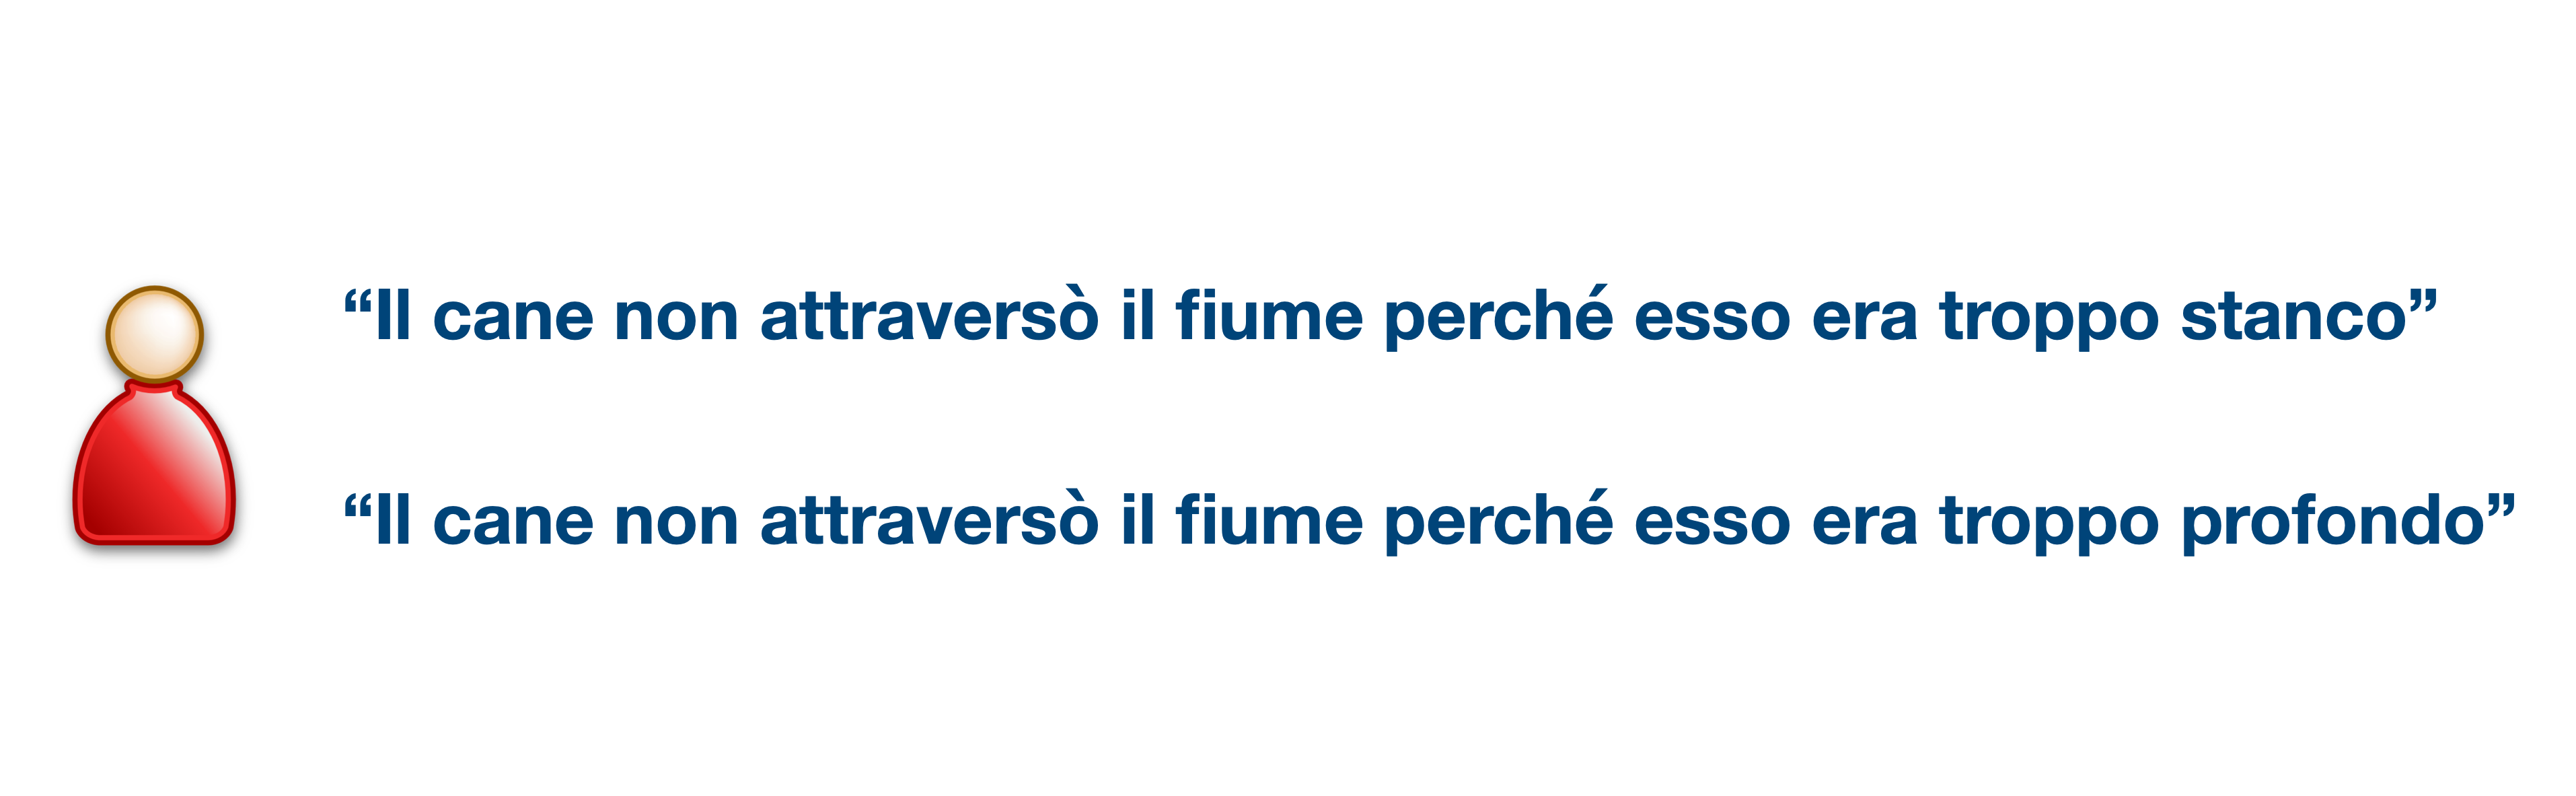
\includegraphics[width=\textwidth]{Context-0.png}
            \end{minipage}
        \end{figure}
    }
    \only<2|handout:0>{
        \begin{figure}[ht]
            \begin{minipage}[b]{0.95\linewidth}
                \centering
                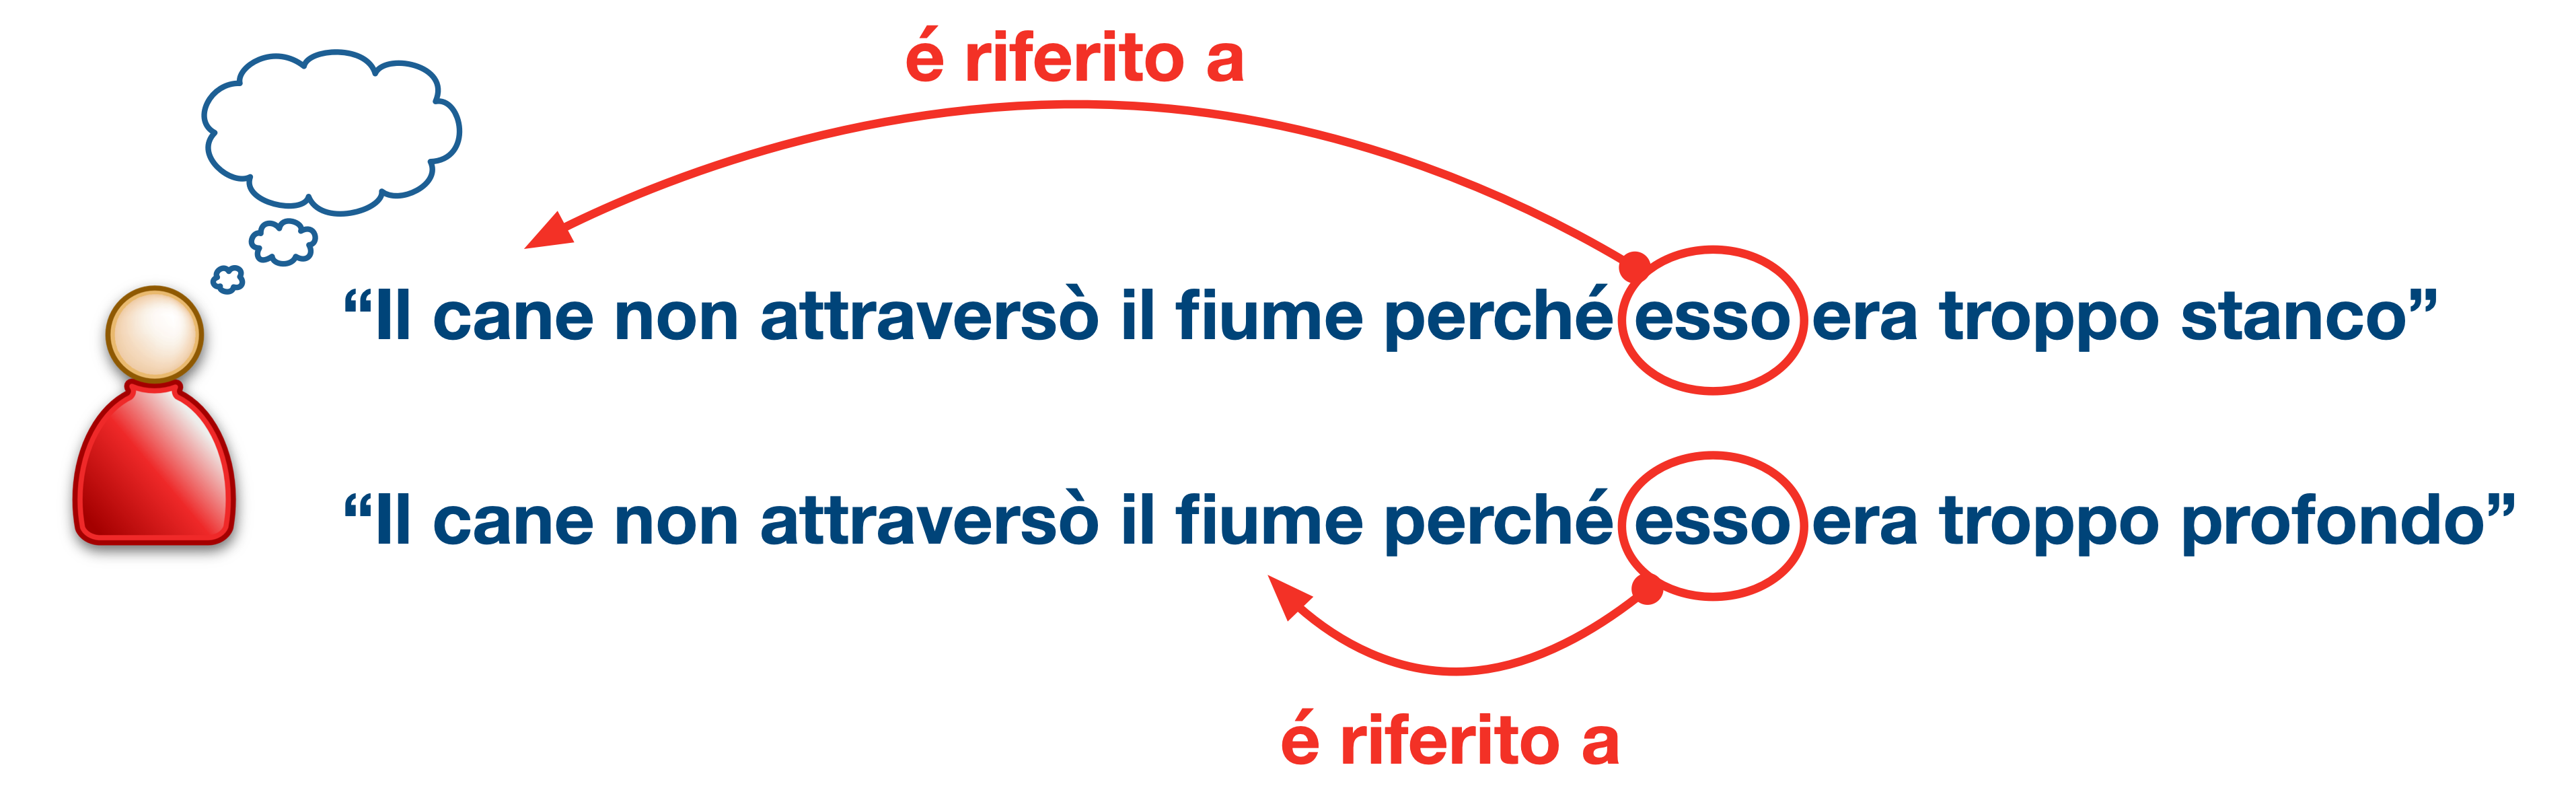
\includegraphics[width=\textwidth]{Context-1.png}
            \end{minipage}
        \end{figure}
    }
    \only<3|handout:1>{
        \begin{figure}[ht]
            \begin{minipage}[b]{0.95\linewidth}
                \centering
                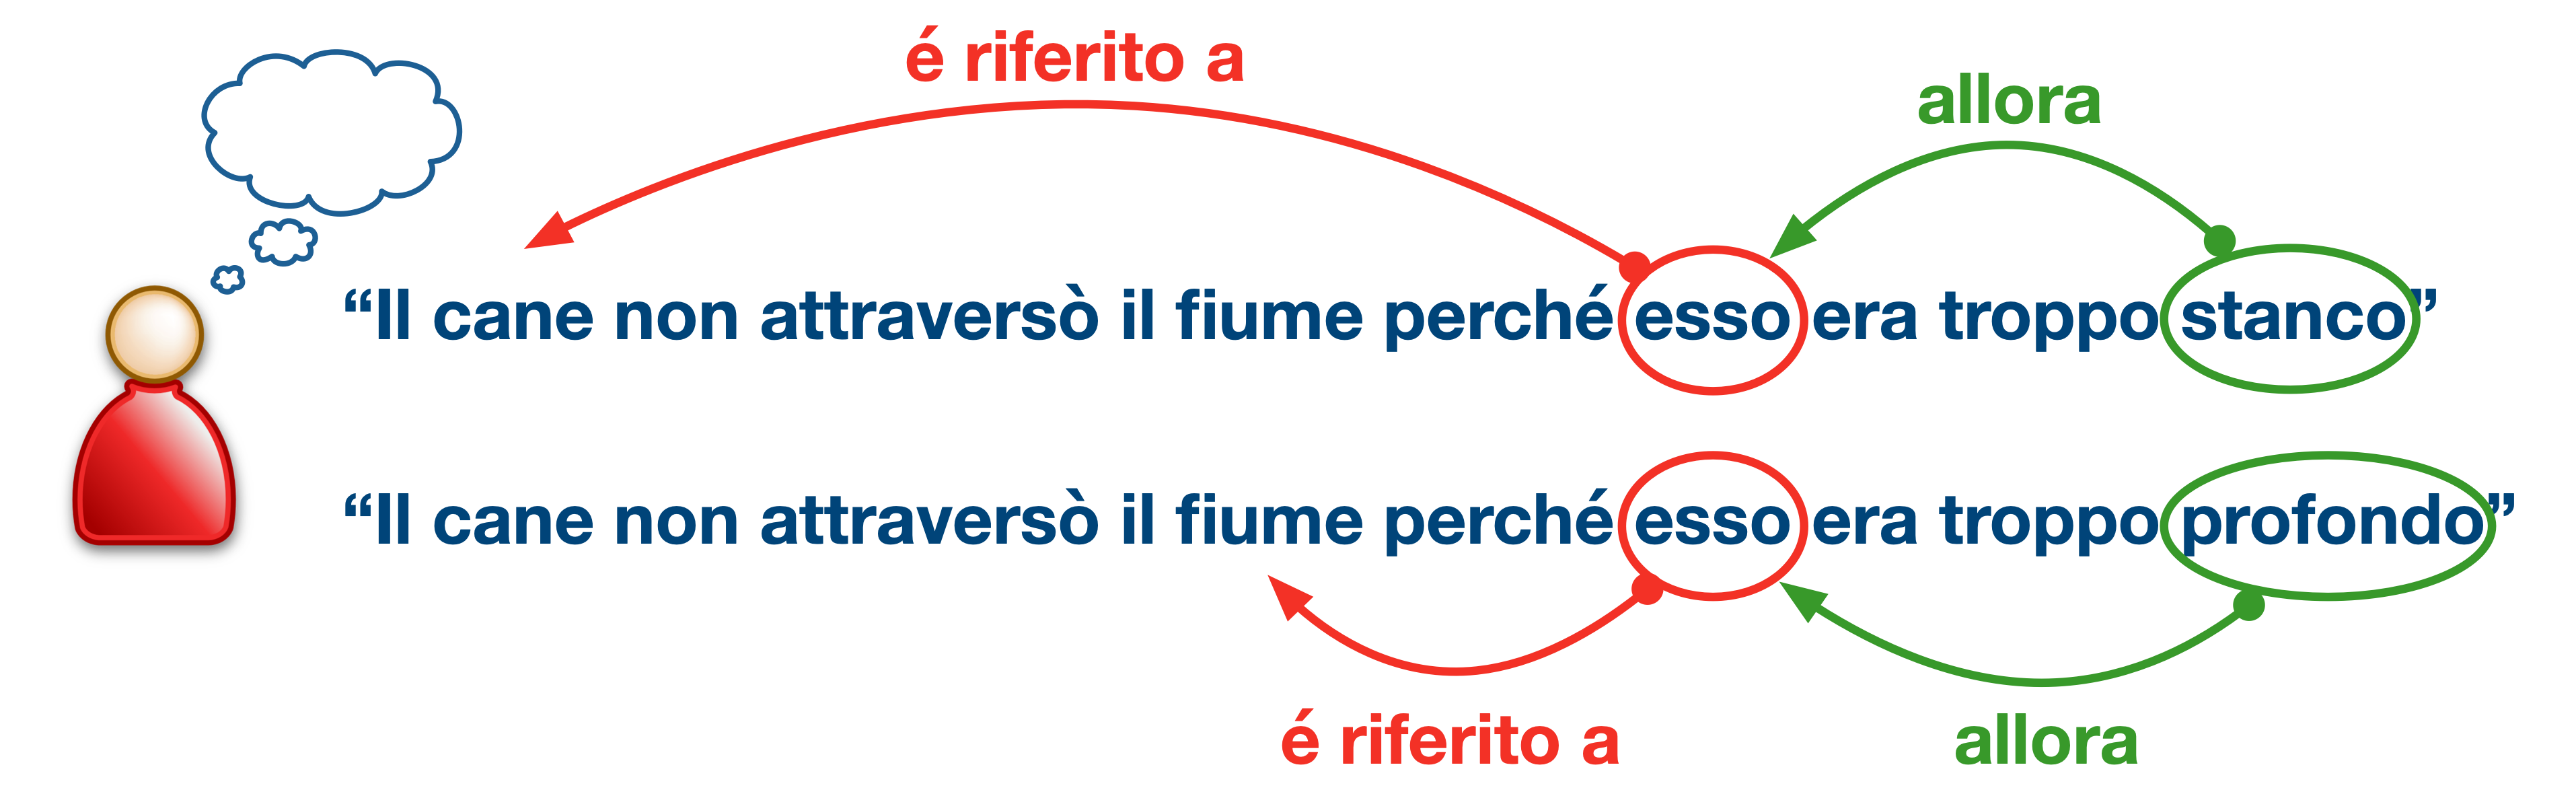
\includegraphics[width=\textwidth]{Context-2.png}
            \end{minipage}
        \end{figure}
    }
    \end{minipage}
        \begin{minipage}[t]{\textwidth}
            \vspace*{.8cm}
            \begin{itemize}[leftmargin=10pt,align=right]
                \onslide<3->\item[\alert{\faArrowCircleRight}] Il significato di alcune parole è dipendente dal significato di altre (\alert{parole contestuali})
                \onslide<4->\item[\alert{\faArrowCircleRight}] L'umano affronta questo processo in maniera inconscia ed istantanea$\ldots$
                \onslide<5->\item[\alert{\faArrowCircleRight}] $\ldots$ ma una macchina?!
            \end{itemize}
        \end{minipage}
    }
\end{frame}
%
\begin{frame}[t,fragile] \frametitle{Le origini: ELIZA (1966)}
    \framesubtitle{Il primo \textit{chatbot} della storia}
	{\small
	    \begin{minipage}[t]{\textwidth}
	    	\begin{itemize}[leftmargin=10pt,align=right]
				\onslide<1->\item[\alert{\faArrowCircleRight}] Sviluppato da \alert{Joseph Weizenbaum} al MIT
				\onslide<2->\item[\alert{\faArrowCircleRight}] Simulava una conversazione con uno \alert{psicoterapeuta} rogersiano
				\onslide<3->\item[\alert{\faArrowCircleRight}] Utilizzava semplici \alert{\textit{pattern matching}} e regole di sostituzione
				\onslide<4->\item[\alert{\faArrowCircleRight}] Dimostrava quanto facilmente le persone potessero essere \alert{ingannate} da un programma semplice
				\onslide<5->\item[\alert{\faArrowCircleRight}] Primo esempio di \alert{illusione di comprensione} da parte di una macchina
			\end{itemize}
        \end{minipage}
		\vfill
		\onslide<1->
		\begin{center}
			\href{https://www.masswerk.at/elizabot/eliza.html}{\faExternalLinkSquare\ Implementazione ELIZA}
		\end{center}
	}
\end{frame}
%
\begin{frame}[t,fragile] \frametitle{ELIZA: come funzionava}
	\framesubtitle{Pattern matching e trasformazioni di template}
	{\small
		\begin{itemize}[leftmargin=10pt,align=right]
			\item[\alert{\faArrowCircleRight}] \alert{Trasformazioni grammaticali:} regole sintattiche applicate all'\textit{input} utente
		\end{itemize}
		\vspace*{.3cm}
		\hspace*{4cm}
		\begin{codeblock}{Regole di trasformazione ELIZA}
        	\begin{minted}{shell-session}
''I am'' -> ''you are''
''my'' -> ''your''
''me'' -> ''you''
...
        	\end{minted}
    	\end{codeblock}
		\hspace*{4cm}
		\begin{minipage}[t]{.6\textwidth}
			\renewcommand{\epigraphsize}{\scriptsize}
			\setlength{\afterepigraphskip}{0pt}
			\setlength{\beforeepigraphskip}{5pt}
			\setlength{\epigraphwidth}{0.9\textwidth}
			\epigraph{\textit{\alert{\faUser} ``\alert{I am} feeling sad today''\\
			\alert{\faTerminal\ (thinking)} --- \alert{you are} feeling sad today---}}{\textbf{ELIZA, elaborazione, 1966}}
		\end{minipage}
	}
\end{frame}
%
\begin{frame}[t,fragile] \frametitle{ELIZA: come funzionava}
	{\small
		\framesubtitle{Pattern matching e trasformazioni di template}
		\begin{itemize}[leftmargin=10pt,align=right]
			\item[\alert{\faArrowCircleRight}] \alert{\textit{Template} di risposta:} frasi predefinite con \textit{slot} per le sostituzioni
		\end{itemize}
		\vspace*{.3cm}
		\hspace*{4cm}
		\begin{codeblock}{Esempi di \textit{template} ELIZA}
        	\begin{minted}{shell-session}
''Tell me more about ___''
''What else comes to mind when ___?''
''Why ___?''
...
        	\end{minted}
    	\end{codeblock}
	}
\end{frame}
%
\begin{frame}[t,fragile] \frametitle{ELIZA: come funzionava}
	\framesubtitle{Pattern matching e trasformazioni di template}
	{\small
		\begin{itemize}[leftmargin=10pt,align=right]
			\item[\alert{\faArrowCircleRight}] \alert{Regole di \textit{pattern matching}:} riconoscimento di parole chiave nell'\textit{input} e scelta fra possibili \textit{pattern} correlati
		\end{itemize}
		\vspace*{.3cm}
		\begin{codeblock}{Esempi di \textit{pattern matching} ELIZA}
        	\begin{minted}{shell-session}
''I think about ___'' -> ''Tell me more about ___''
''I am thinking of ___'' -> ''What else comes to mind when you think of ___?''
''I am ___'' -> ''Why do you think ___?''
...
        	\end{minted}
    	\end{codeblock}
		\hspace*{4cm}
		\begin{minipage}[t]{.6\textwidth}
			\renewcommand{\epigraphsize}{\scriptsize}
			\setlength{\afterepigraphskip}{0pt}
			\setlength{\beforeepigraphskip}{5pt}
			\setlength{\epigraphwidth}{0.9\textwidth}
			\epigraph{\textit{\alert{\faUser} ``\alert{I am} feeling sad today''\\
			\alert{\faTerminal} ``Why do you think you are feeling sad today?''}}{\textbf{ELIZA, esempio di risposta, 1966}}
		\end{minipage}
	}
\end{frame}
%
\begin{frame}[t,fragile] \frametitle{ELIZA: come funzionava}
	\framesubtitle{Pattern matching e trasformazioni di template}
	{\small
		\begin{itemize}[leftmargin=10pt,align=right]
			\item[\alert{\faArrowCircleRight}] \alert{Strategia di \textit{fallback}:} formule generiche quando non trova \textit{pattern}
		\end{itemize}
		\vspace*{.3cm}
		\hspace*{4cm}
		\begin{minipage}[t]{.6\textwidth}
			\renewcommand{\epigraphsize}{\scriptsize}
			\setlength{\afterepigraphskip}{0pt}
			\setlength{\beforeepigraphskip}{5pt}
			\setlength{\epigraphwidth}{0.9\textwidth}
			\epigraph{\textit{\alert{\faUser} ``\alert{My} whole world is falling apart.''\\
			\alert{\faTerminal} ``I see.''\\
			(oppure)\\
			\alert{\faTerminal} ``Can you elaborate on that?''\\
			(oppure)\\
			\alert{\faTerminal} ``I see.''\\
			(oppure)\\
			\alert{\faTerminal} ``What does that suggest to you?''\\
			(oppure)\\
			\alert{\faTerminal} ``Please go on.''\\
			(oppure)\\
			\alert{\faTerminal} ``How does that make you feel?''
			}}{\textbf{ELIZA, esempio di risposta, 1966}}
		\end{minipage}
	}
\end{frame}
%
\begin{frame}[t,fragile] \frametitle{Bag-of-Words}
    \framesubtitle{Rappresentazione testo non strutturato}
	{\small
		\begin{minipage}[t]{\textwidth}
	    	\begin{itemize}[leftmargin=10pt,align=right]
				\onslide<1->\item[\alert{\faArrowCircleRight}] Menzionato per la prima volta negli anni '50, popolare negli anni 2000
				\onslide<2->\item[\alert{\faArrowCircleRight}] Metodo per rappresentare il testo \alert{non strutturato} in formato numerico
				\onslide<3->\item[\alert{\faArrowCircleRight}] Il \alert{linguaggio è complicato} per i calcolatori
				\begin{itemize}[leftmargin=10pt,align=right]
					\item[\alert{\faArrowCircleRight}] Il testo perde significato quando rappresentato da 0 e 1
				\end{itemize}
				\onslide<4->\item[\alert{\faArrowCircleRight}] \alert{\textit{Focus} principale:} rappresentare il linguaggio in \alert{modo strutturato} per l'uso da parte dei calcolatori
			\end{itemize}
        \end{minipage}
	}
\end{frame}
%
\begin{frame}[t,fragile] \frametitle{Bag-of-Words: come funziona}
	\framesubtitle{Processo di tokenizzazione e creazione del vocabolario}
	{\footnotesize
		\begin{itemize}[leftmargin=10pt,align=right]
			\onslide<1->{\item[\alertedcircled{1}] \alert{Tokenizzazione:} processo di divisione delle frasi in parole individuali o sotto-parole (\alert{\textit{token}})
			\begin{itemize}[leftmargin=10pt,align=right]
				\item[\alert{\faArrowCircleRight}] Rispetto a un \alert{delimitatore} (specifico o \textit{wildcard}) e una \alert{\textit{blacklist}}
			\end{itemize}}
			\onslide<2->{\item[\alertedcircled{2}] \alert{Creazione del vocabolario:} estrazione di entità uniche dai \textit{token}
			\begin{itemize}[leftmargin=10pt,align=right]
				\item[\alert{\faArrowCircleRight}] Applicando estrazione della radice (\alert{\textit{stemming}})
				\item[\alert{\faExclamationTriangle}] Vettore \alert{ordinato} di radici
			\end{itemize}}
			\onslide<3->{\item[\alertedcircled{3}] \alert{Conteggio delle parole:} rappresentazione numerica basata sulla \alert{frequenza}}
		\end{itemize}
		\hspace*{1cm}
		\only<1|handout:1>{
			\begin{minipage}[t]{.9\textwidth}
				{\tiny
					\begin{table}
						\setlength{\tabcolsep}{4pt}
						\renewcommand{\arraystretch}{1}
						\begin{tabular}{c|c|c|c|c|c|c|c|c|c|c|c}
							\multicolumn{12}{c}{\textbf{Token}}\\
							\midrule
							che & bel & cane & che & hai & ma & il & mio & gatto & è & più & bello\\
							\midrule
						\end{tabular}
					\end{table}
				}
				\renewcommand{\epigraphsize}{\scriptsize}
				\setlength{\afterepigraphskip}{0pt}
				\setlength{\beforeepigraphskip}{0pt}
				\setlength{\epigraphwidth}{0.9\textwidth}
				\epigraph{\textit{\alert{\faFile$_1$} ``Che\,\Vtextvisiblespace[1em]\,bel\,\Vtextvisiblespace\,cane\,\Vtextvisiblespace[1cm]\,che\,\Vtextvisiblespace[.5em]\,hai!''\\
				\alert{\faFile$_2$} ``Ma\,\Vtextvisiblespace[.3cm]\,il\,\Vtextvisiblespace[1cm]\,mio\,\Vtextvisiblespace[.1cm]\,gatto\,\Vtextvisiblespace[1em]\,è\,\Vtextvisiblespace[.5em]\,più\,\Vtextvisiblespace[1cm]\,bello''}
}{\textbf{Tokenizzazione}}
			\end{minipage}
		}
		\only<2|handout:2>{
			\begin{minipage}[t]{.9\textwidth}
				{\tiny
					\begin{table}
						\setlength{\tabcolsep}{4pt}
						\renewcommand{\arraystretch}{1}
						\begin{tabular}{c|c|c|c|c|c|c|c|c|c|c}
							\multicolumn{11}{c}{\textbf{Vocabolario}}\\
							\midrule
							che & bell- & can- & avere & ma & il & mi- & gatt- & essere & più & bell-\\
							\midrule
						\end{tabular}
					\end{table}
				}
				\renewcommand{\epigraphsize}{\scriptsize}
				\setlength{\afterepigraphskip}{0pt}
				\setlength{\beforeepigraphskip}{0pt}
				\setlength{\epigraphwidth}{0.9\textwidth}
				\epigraph{\textit{\alert{\faFile$_1$} ``Che\,\Vtextvisiblespace[1em]\,bel\,\Vtextvisiblespace\,cane\,\Vtextvisiblespace[1cm]\,che\,\Vtextvisiblespace[.5em]\,hai!''\\
				\alert{\faFile$_2$} ``Ma\,\Vtextvisiblespace[.3cm]\,il\,\Vtextvisiblespace[1cm]\,mio\,\Vtextvisiblespace[.1cm]\,gatto\,\Vtextvisiblespace[1em]\,è\,\Vtextvisiblespace[.5em]\,più\,\Vtextvisiblespace[1cm]\,bello''
				}
				}{\textbf{Creazione del vocabolario}}
			\end{minipage}
		}
		\only<3|handout:3>{
			\begin{minipage}[t]{.9\textwidth}
				{\tiny
					\begin{table}
						\setlength{\tabcolsep}{4pt}
						\renewcommand{\arraystretch}{1}
						\begin{tabular}{cc|c|c|c|c|c|c|c|c|c|c}
							& \multicolumn{11}{c}{\textbf{Vocabolario}}\\
							\cmidrule{2-12}
				        	& che & bell- & can- & avere & ma & il & mi- & gatt- & essere & più & bell-\\
							\cmidrule{2-12}
							\alert{\faFile$_1$} & 2   & 1   & 1    & 1     & 0  & 0  & 0   & 0     & 0      & 0   & 0    \\
							\alert{\faFile$_2$} & 0   & 0   & 0    & 0     & 1  & 1  & 1   & 1     & 1      & 1   & 1    \\
							\cmidrule{2-12}
						\end{tabular}
					\end{table}
				}
				\renewcommand{\epigraphsize}{\scriptsize}
				\setlength{\afterepigraphskip}{0pt}
				\setlength{\beforeepigraphskip}{0pt}
				\setlength{\epigraphwidth}{0.9\textwidth}
				\epigraph{\textit{\alert{\faFile$_1$} ``Che\,\Vtextvisiblespace[1em]\,bel\,\Vtextvisiblespace\,cane\,\Vtextvisiblespace[1cm]\,che\,\Vtextvisiblespace[.5em]\,hai!''\\
				\alert{\faFile$_2$} ``Ma\,\Vtextvisiblespace[.3cm]\,il\,\Vtextvisiblespace[1cm]\,mio\,\Vtextvisiblespace[.1cm]\,gatto\,\Vtextvisiblespace[1em]\,è\,\Vtextvisiblespace[.5em]\,più\,\Vtextvisiblespace[1cm]\,bello''
				}}{\textbf{Vettori \textit{bag-of-words}}}
		\end{minipage}
		}	
	}
\end{frame}
%
\begin{frame}[t,fragile] \frametitle{Bag-of-Words}
	\framesubtitle{Limitazioni}
	{\small
		\begin{itemize}[leftmargin=10pt,align=right]
			\onslide<1->{\item[\alert{\faArrowCircleRight}] \alert{Perdita dell'ordine:} frasi diammetralmente opposte hanno la medesima rappresentazione}
			\onslide<2->{\item[\alert{\faArrowCircleRight}] \alert{Mancanza di semantica:} Non cattura il significato delle parole
			\item[\alert{\faArrowCircleRight}] \alert{Nessuna generalizzazione:} i sinonimi sono trattati come elementi \alert{totalmente separati}}
			\onslide<3->{\item[\alert{\faArrowCircleRight}] \alert{Alta dimensionalità:} Vocabolari enormi con molti zeri}
		\end{itemize}
		\hspace*{2cm}
		\only<1|handout:1>{
		\begin{minipage}[t]{.75\textwidth}
		{\tiny
		\begin{table}
			\setlength{\tabcolsep}{4pt}
			\renewcommand{\arraystretch}{1}
			\begin{tabular}{cc|c|c|c}
								& \multicolumn{3}{c}{\textbf{Vocabolario}}\\
				\cmidrule{2-5}
				        & Simone & mangiare & l- & insalat-\\
				\cmidrule{2-5}
				\alert{\faFile$_1$} & 1   & 1   & 1    & 1\\
				\alert{\faFile$_2$} & 1   & 1   & 1    & 1\\
				\midrule
			\end{tabular}
		\end{table}
		}
			\renewcommand{\epigraphsize}{\scriptsize}
			\setlength{\afterepigraphskip}{0pt}
			\setlength{\beforeepigraphskip}{0pt}
			\setlength{\epigraphwidth}{0.9\textwidth}
			\epigraph{\textit{\alert{\faFile$_1$} ``Simone\,\Vtextvisiblespace[1em]\,mangiò\,\Vtextvisiblespace[1em]\,l'\,\Vtextvisiblespace[1em]\,insalata''\\
			\alert{\faFile$_2$} ``L'\,\Vtextvisiblespace[1em]\,insalata\,\Vtextvisiblespace[1em]\,mangiò\,\Vtextvisiblespace[1em]\,Simone''}}{\textbf{Problema dell'ordine delle parole}}
		\end{minipage}
		}
		\only<2|handout:2>{
		\begin{minipage}[t]{.75\textwidth}
			\renewcommand{\epigraphsize}{\scriptsize}
			\setlength{\afterepigraphskip}{0pt}
			\setlength{\beforeepigraphskip}{5pt}
			\setlength{\epigraphwidth}{0.9\textwidth}
			\epigraph{\textit{\alert{\faUser} ``Concetti come <<Re>> e <<Regina>> dovrebbero essere correlati\ldots''\\
			\alert{\faUser} ``Sinonimi come <<felice>> e <<gioioso>> dovrebbero avere una rappresentazione simile\ldots''\\
			\alert{\faUser} ``E con parole come <<pitone>> e <<serpente>>, una generalizzazione dell'altra?!''}}{\textbf{Mancanza di relazioni semantiche}}
		\end{minipage}
		}
		\only<3|handout:3>{
		\begin{minipage}[t]{.75\textwidth}
			\renewcommand{\epigraphsize}{\scriptsize}
			\setlength{\afterepigraphskip}{0pt}
			\setlength{\beforeepigraphskip}{5pt}
			\setlength{\epigraphwidth}{0.9\textwidth}
			\epigraph{\textit{\alert{\faUser} ``Fornisci una stima del vocabolario usato in Wikipedia.''\\
			\alert{\faTerminal} ``[\ldots] English Wikipedia: ordine di grandezza \alert{$10^5$--$10^7$} [\ldots]. Tutte le Wikipedie insieme (tutte le lingue, forme di parola): ordine di grandezza \alert{$10^5$--$10^8$} [\ldots].\\
			\alert{\faUser:} ``Quindi un documento Wikipedia in Bag-Of-Words sarebbe rappresentato da un vettore di dimensione almeno \alert{$10^5$}?!''}}{\textbf{Problema della dimensionalità}}
		\end{minipage}
		}
	}
\end{frame}
%
\begin{frame}[t,fragile] \frametitle{Word Embeddings (2013)}
	\framesubtitle{Word2Vec e le rappresentazioni dense}
	    \begin{minipage}[t]{\textwidth}
	    	\begin{itemize}[leftmargin=10pt,align=right]
				\onslide<1->\item[\alert{\faArrowCircleRight}] \alert{Word2Vec:} primo tentativo di successo per catturare il significato del testo negli \textit{embeddings}
				\onslide<2->\item[\alert{\faArrowCircleRight}] \alert{\textit{Embeddings}:} rappresentazioni vettoriali di dati che tentano di catturarne il significato
				\onslide<3->\item[\alert{\faArrowCircleRight}] Addestrato su \alert{enormi quantità} di dati testuali
				\begin{itemize}[leftmargin=10pt,align=right]
					\item[\alert{\faArrowCircleRight}] British National Corpus
					\item[\alert{\faArrowCircleRight}] English Wikipedia
					\item[\alert{\faArrowCircleRight}] Google News
					\item[\alert{\faArrowCircleRight}] English Gigaword
					\item[\alert{\faArrowCircleRight}] \ldots
				\end{itemize}
				\onslide<4->\item[\alert{\faArrowCircleRight}] Utilizza \alert{reti neurali} per generare rappresentazioni semantiche
				\onslide<5->\item[\alert{\faExclamationTriangle}] Grandezza della rappresentazione vettoriale \alert{limitata a priori}
			\end{itemize}
	    \end{minipage}
\end{frame}
%
\begin{frame}[t,fragile] \frametitle{Word2Vec: come funziona}
	\framesubtitle{Apprendimento delle relazioni tra parole}
	{\footnotesize
		\begin{itemize}[leftmargin=10pt,align=right]
			\onslide<1->{\item[\alert{\faArrowCircleRight}] \alert{Principio fondamentale:} parole che appaiono in contesti simili tendono ad avere significati simili}
			\onslide<2->{\item[\alert{\faArrowCircleRight}] \alert{Addestramento:} predire se due parole sono vicine in una frase}
			\onslide<3->{\item[\alert{\faArrowCircleRight}] \alert{Risultato:} parole con significati simili hanno \textit{embeddings} vicini nello spazio}
		\end{itemize}
		\hspace*{3cm}
		\only<1|handout:1>{
		\begin{minipage}[t]{.7\textwidth}
			\renewcommand{\epigraphsize}{\scriptsize}
			\setlength{\afterepigraphskip}{0pt}
			\setlength{\beforeepigraphskip}{5pt}
			\setlength{\epigraphwidth}{0.9\textwidth}
			\epigraph{\textit{\alert{\faFile$_1$} ``[\ldots] Il mio cane ama dormire nella sua cuccia [\ldots]''\\
			\alert{\faFile$_2$} ``[\ldots] Il \alert{veterinario} ha deciso di sterilizzare il gatto [\ldots]''\\
			\alert{\faFile$_3$} ``[\ldots] Mentre giocava, il mio cane si è fatto male e l'ho dovuto portare dal veterinario [\ldots]''\\
			\alert{\faFile$_4$} ``[\ldots] Ho comprato una cuccia per il mio gatto, ma continua a preferire il divano! [\ldots]''\\
			\alert{\faTerminal\ (thinking)} --- Devo capire quali termini condividono gli stessi contesti linguistici\ldots ---}}{\textbf{Principio alla base di Word2Vec}}
			%
			\epigraph{\textit{You shall know a word by the company it keeps.}}{\textbf{Ipotesi distributiva, John Rupert Firth, 1957}}
		\end{minipage}
		}
		\only<2|handout:2>{
		\begin{minipage}[t]{.7\textwidth}
			\renewcommand{\epigraphsize}{\scriptsize}
			\setlength{\afterepigraphskip}{0pt}
			\setlength{\beforeepigraphskip}{5pt}
			\setlength{\epigraphwidth}{0.9\textwidth}
			\epigraph{\textit{\alert{\faFile$_1$} ``[\ldots] Il mio \alert{cane} ama dormire nella sua \alert{cuccia} [\ldots]''\\
			\alert{\faFile$_2$} ``[\ldots] Il \textit{veterinario} ha preferito sterilizzare il \alert{gatto} [\ldots]''\\
			\alert{\faFile$_3$} ``[\ldots] Mentre giocava, il mio \alert{cane} si è fatto male e l'ho dovuto portare dal \alert{veterinario} [\ldots]''\\
			\alert{\faFile$_4$} ``[\ldots] Ho comprato una \alert{cuccia} per il mio \alert{gatto}, ma continua a preferire il divano! [\ldots]''\\
			\alert{\faTerminal\ (thinking)} --- Devo avvicinare le rappresentazioni di <<cane>> e <<gatto>> nello spazio perché condividono spesso gli stessi vicini <<veterinario>> e <<cuccia>>! ---}}{\textbf{Addestramento di Word2Vec}}
		\end{minipage}
		}
		\only<3|handout:3>{
		\begin{minipage}[t]{.7\textwidth}
			\renewcommand{\epigraphsize}{\scriptsize}
			\setlength{\afterepigraphskip}{0pt}
			\setlength{\beforeepigraphskip}{5pt}
			\setlength{\epigraphwidth}{0.9\textwidth}
			\epigraph{\textit{\alert{\faTerminal} ``<<Computer>> è simile a <<laptop>>, <<pc>>, <<desktop>>, <<workstation>>, \ldots''\\	
			\alert{\faTerminal} ``<<Re>> sta a <<uomo>> come <<Regina>> sta a <<donna>>!''\\
			\alert{\faTerminal} ``<<Lunedì>>, <<martedì>>, <<mercoledì>>, \ldots formano un unico gruppo.''}}{\textbf{Proprietà emergenti: sinonimie, classificazioni, relazionalità}}
			\begin{center}
				\href{https://vectors.nlpl.eu/explore/embeddings/en/}{\faExternalLinkSquare\ Portale Word2Vec}
			\end{center}
		\end{minipage}
		}
	}
\end{frame}
%
\begin{frame}[t,fragile] \frametitle{Word2Vec}
	\framesubtitle{Limitazioni}
		\begin{itemize}[leftmargin=10pt,align=right]
			\onslide<1->{\item[\alert{\faArrowCircleRight}] \alert{Polisemia:} confusione con parole utilizzabili con diversi significati in contesti diversi}
			\onslide<2->{\item[\alert{\faArrowCircleRight}] \alert{Contesti insufficienti:} parole rare potrebbero non avere abbastanza esempi}
		\end{itemize}
		\hspace*{3cm}
		\only<1|handout:1>{
		\begin{minipage}[t]{.7\textwidth}
			\renewcommand{\epigraphsize}{\scriptsize}
			\setlength{\afterepigraphskip}{5pt}
			\setlength{\beforeepigraphskip}{5pt}
			\setlength{\epigraphwidth}{0.9\textwidth}
			\epigraph{\alert{\faTerminal\ (thinking)} --- Ma\ldots <<cannonata>> in senso bellico\ldots O calcistico? ---}{\textbf{Problema della polisemia}}
		\end{minipage}
		}
		\only<2|handout:2>{
		\begin{minipage}[t]{.7\textwidth}
			\renewcommand{\epigraphsize}{\scriptsize}
			\setlength{\afterepigraphskip}{5pt}
			\setlength{\beforeepigraphskip}{5pt}
			\setlength{\epigraphwidth}{0.9\textwidth}
			\epigraph{\textit{\alert{\faTerminal\ (thinking)} --- Non ho molto capito il senso delle parole <<supercazzola>>, <<scappellamento>> e <<Antani>>\ldots ---}}{\textbf{Amici miei, 1975}}
		\end{minipage}
		}
\end{frame}
